\PassOptionsToPackage{unicode=true}{hyperref} % options for packages loaded elsewhere
\PassOptionsToPackage{hyphens}{url}
\PassOptionsToPackage{dvipsnames,svgnames*,x11names*}{xcolor}
%
\documentclass[10pt,ignorenonframetext,]{beamer}
\usepackage{pgfpages}
\setbeamertemplate{caption}[numbered]
\setbeamertemplate{caption label separator}{: }
\setbeamercolor{caption name}{fg=normal text.fg}
\beamertemplatenavigationsymbolsempty
% Prevent slide breaks in the middle of a paragraph:
\widowpenalties 1 10000
\raggedbottom
\setbeamertemplate{part page}{
\centering
\begin{beamercolorbox}[sep=16pt,center]{part title}
  \usebeamerfont{part title}\insertpart\par
\end{beamercolorbox}
}
\setbeamertemplate{section page}{
\centering
\begin{beamercolorbox}[sep=12pt,center]{part title}
  \usebeamerfont{section title}\insertsection\par
\end{beamercolorbox}
}
\setbeamertemplate{subsection page}{
\centering
\begin{beamercolorbox}[sep=8pt,center]{part title}
  \usebeamerfont{subsection title}\insertsubsection\par
\end{beamercolorbox}
}
\AtBeginPart{
  \frame{\partpage}
}
\AtBeginSection{
  \ifbibliography
  \else
    \frame{\sectionpage}
  \fi
}
\AtBeginSubsection{
  \frame{\subsectionpage}
}
\usepackage{lmodern}
\usepackage{amssymb,amsmath}
\usepackage{ifxetex,ifluatex}
\usepackage{fixltx2e} % provides \textsubscript
\ifnum 0\ifxetex 1\fi\ifluatex 1\fi=0 % if pdftex
  \usepackage[T1]{fontenc}
  \usepackage[utf8]{inputenc}
  \usepackage{textcomp} % provides euro and other symbols
\else % if luatex or xelatex
  \usepackage{unicode-math}
  \defaultfontfeatures{Ligatures=TeX,Scale=MatchLowercase}
\fi
\usetheme[]{Singapore}
\usefonttheme{serif}
% use upquote if available, for straight quotes in verbatim environments
\IfFileExists{upquote.sty}{\usepackage{upquote}}{}
% use microtype if available
\IfFileExists{microtype.sty}{%
\usepackage[]{microtype}
\UseMicrotypeSet[protrusion]{basicmath} % disable protrusion for tt fonts
}{}
\IfFileExists{parskip.sty}{%
\usepackage{parskip}
}{% else
\setlength{\parindent}{0pt}
\setlength{\parskip}{6pt plus 2pt minus 1pt}
}
\usepackage{xcolor}
\usepackage{hyperref}
\hypersetup{
            pdftitle={Linear regresjon (enkel og multippel)},
            pdfauthor={Stefanie Muff, Institutt for matematiske fag},
            colorlinks=true,
            linkcolor=Maroon,
            filecolor=Maroon,
            citecolor=Blue,
            urlcolor=blue,
            breaklinks=true}
\urlstyle{same}  % don't use monospace font for urls
\newif\ifbibliography
\usepackage{graphicx,grffile}
\makeatletter
\def\maxwidth{\ifdim\Gin@nat@width>\linewidth\linewidth\else\Gin@nat@width\fi}
\def\maxheight{\ifdim\Gin@nat@height>\textheight\textheight\else\Gin@nat@height\fi}
\makeatother
% Scale images if necessary, so that they will not overflow the page
% margins by default, and it is still possible to overwrite the defaults
% using explicit options in \includegraphics[width, height, ...]{}
\setkeys{Gin}{width=\maxwidth,height=\maxheight,keepaspectratio}
\setlength{\emergencystretch}{3em}  % prevent overfull lines
\providecommand{\tightlist}{%
  \setlength{\itemsep}{0pt}\setlength{\parskip}{0pt}}
\setcounter{secnumdepth}{0}

% set default figure placement to htbp
\makeatletter
\def\fps@figure{htbp}
\makeatother

\usepackage{multicol}

\title{Linear regresjon (enkel og multippel)}
\providecommand{\subtitle}[1]{}
\subtitle{ISTx1003 Statistisk læring og Data Science}
\author{Stefanie Muff, Institutt for matematiske fag}
\date{November 1 og 5, 2021}

\begin{document}
\frame{\titlepage}

\begin{frame}{Anerkjennelse}
\protect\hypertarget{anerkjennelse}{}

\(~\)

Disse slides bygger på slides fra Mette Langaas, 2020.

Takk til Mette for at jeg fikk bruke noen av materialene.

\end{frame}

\begin{frame}{Plan for i dag og fredag 12:15-13:00 (tema ``Regresjon'')}
\protect\hypertarget{plan-for-i-dag-og-fredag-1215-1300-tema-regresjon}{}

\(~\)

\begin{itemize}
\item
  Læringsmål og plan for prosjektmodulen ISTx1003.
\item
  De tre temaene i modulen:

  \begin{itemize}
  \tightlist
  \item
    regresjon
  \item
    klassifikasjon og
  \item
    klyngeananlyse
  \end{itemize}
\item
  Pensum og læringsressurser
\item
  Prosjektoppgaven og Blackboard-informasjon
\item
  Tema: Enkel og multippel lineær regresjon
\end{itemize}

\end{frame}

\begin{frame}{Hvem er vi?}
\protect\hypertarget{hvem-er-vi}{}

\(~\)

\begin{itemize}
\item
  \textbf{Studentene}: BIDATA og BDIGSEC, omtrent 250 studenter totalt.
\item
  \textbf{Faglig ansvarlig} for innholdet i modulen er Stefanie Muff
  (\href{mailto:stefanie.muff@ntnu.no}{\nolinkurl{stefanie.muff@ntnu.no}}).
\item
  I \textbf{veilederteamet} (for prosjektet) inngår i tillegg

  \begin{itemize}
  \tightlist
  \item
    Trondheim: studentassistentene Simen, Simon og Philip, og
    øvingslærer Martin O. Berild
  \item
    Gjøvik: Charles Curry \ldots{}
  \item
    Ålesund: Siebe B. van Albada, \ldots{}
  \end{itemize}
\end{itemize}

\end{frame}

\begin{frame}{Hva er statistisk læring og data science?}
\protect\hypertarget{hva-er-statistisk-luxe6ring-og-data-science}{}

\(~\)

\begin{itemize}
\tightlist
\item
  \emph{Statistisk læring} inneholder stort sett alle metoder som
  hjelper oss å lære av data.
\end{itemize}

\vspace{2mm}

\begin{itemize}
\tightlist
\item
  \emph{Data science} er et konsept for å forene statistikk,
  dataanalyse, informatikk og tilhørende metoder for å "forstå og
  analysere relle fenomener med data.
\end{itemize}

\end{frame}

\begin{frame}{Læringsmål (av modulen)}
\protect\hypertarget{luxe6ringsmuxe5l-av-modulen}{}

Etter du har gjennomført denne modulen skal du kunne:

\begin{itemize}
\item
  forstå når du kan bruke regresjon, klassifikasjon og klyngeananlyse
  til å løse et ingeniørproblem
\item
  kunne gjennomføre multippel lineær regresjon på et datasett
\item
  bruke logistisk regresjon og nærmeste nabo for å utføre en
  klassifikasjonsoppgave
\item
  bruke hierarkisk og \(k\)-means klyngeanalyse på et datasett, forstå
  begrepet avstandsmål
\item
  og kunne kommunisere resultatene fra regresjon/
  klassifikasjon/klyngeanalyse til medstudenter og ingeniører
\item
  bli en kritisk leser av resultater fra statistikk/maskinlæring/
  statistisk læring/data science/kunstig intelligens når disse
  rapporteres i media, og forstå om resultatene er realistiske ut fra
  informasjonen som gis
\item
  kunne besvare prosjektoppgaven på en god måte!
\end{itemize}

\end{frame}

\begin{frame}{Pensum og læringsressurser}
\protect\hypertarget{pensum-og-luxe6ringsressurser}{}

Pensum er definert som ``svarene på det du blir spurt om på
prosjektoppgaven'' og de kan du finne ved å bruke læringsressursene.

\vspace{2mm}

Alle ressurser er tilgjengelig her:

\url{https://wiki.math.ntnu.no/istx1003/2021h/start}

\(~\)

Tema Regresjon:

\vspace{2mm}

\begin{itemize}
\item
  \textbf{Kompendium}: Regresjon (pdf og html, by Mette Langaas)
\item
  \textbf{Korte videoer}: (by Mette Langaas)

  \begin{itemize}
  \tightlist
  \item
    Multippel lineær regresjon: introduksjon (14:07 min)
  \item
    Multippel lineær regresjon: analyse av et datasett (15:20 min)
  \end{itemize}
\item
  Denne forelesningen
\item
  \textbf{Disse slides} med notater
\end{itemize}

\end{frame}

\begin{frame}{Prosjektoppgaven}
\protect\hypertarget{prosjektoppgaven}{}

\(~\)

\begin{itemize}
\tightlist
\item
  Vi ser hvor informasjonen ligger på Blackboard og hvordan melde seg på
  gruppe.
\end{itemize}

\vspace{2mm}

\begin{itemize}
\tightlist
\item
  Vi ser på prosjektoppgaven på \url{https://s.ntnu.no/isthub}.
\end{itemize}

\vspace{2mm}

\begin{itemize}
\tightlist
\item
  Karakteren teller 30\% til den endelige karakteren.
\end{itemize}

\vspace{2mm}

\begin{itemize}
\tightlist
\item
  Vi bruker prosentvurderingsmetoden: Konverterer poengene i en \%
  (heltall, avrundet) og så bruker vi følgende skala:
\end{itemize}

\centering

\includegraphics[width=0.4\textwidth,height=\textheight]{prosent.png}

\end{frame}

\begin{frame}{Veileding til prosjektoppgaven}
\protect\hypertarget{veileding-til-prosjektoppgaven}{}

\(~\)

\textbf{Trondheim}: 11., 18. og 25. November, 12:15-14:00 i Sentralbygg
S3.

\textbf{Ålesund}:

\textbf{Gjøvik}:

\end{frame}

\begin{frame}{Læringsmål for regresjon}
\protect\hypertarget{luxe6ringsmuxe5l-for-regresjon}{}

\(~\)

\begin{itemize}
\tightlist
\item
  Du kan lage en modell for å forstå sammenhengen mellom en respons og
  én eller flere forklaringsvariabler.
\end{itemize}

\(~\)

\begin{itemize}
\tightlist
\item
  Du kan lage en modell for å predikere en respons fra en eller flere
  forklaringsvariabler.
\end{itemize}

\end{frame}

\begin{frame}{Regresjon -- motiverende eksempel}
\protect\hypertarget{regresjon-motiverende-eksempel}{}

\centering\tiny(Veiledet læring - vi kjenner responsen)

\vspace{2mm}

\flushleft
\normalsize

\begin{itemize}
\tightlist
\item
  Kropssfett er en viktig indikator for overvekt, men vanskelig å måle.
\end{itemize}

\vspace{2mm}

\textbf{Spørsmål:} Hvilke faktorer tillater præsis estimering av
kroppsfettet?

\vspace{2mm}

Vi undersøker 243 mannlige deltakere. Kroppsfett (\%), BMI og andre
forklaringsvariabler ble målet. Kryssplott:

\begin{center}\includegraphics[width=1\linewidth]{1Regresjon_files/figure-beamer/motivating-1} \end{center}

\end{frame}

\begin{frame}

For en model for funker god for prediksjon trenger vi \emph{multippel
linear regresjon}. Men vi begynner med \emph{enkel linear regresjon}
(bare en forklaringsvariabel):

\begin{center}\includegraphics[width=0.7\linewidth]{1Regresjon_files/figure-beamer/motivating2-1} \end{center}

\end{frame}

\begin{frame}{Enkel linear regresjon}
\protect\hypertarget{enkel-linear-regresjon}{}

\(~\)

\begin{itemize}
\item
  En kontinuerlig respons variabel \(Y\)
\item
  Bare \emph{en forklaringsvariabel} \(x_1\)
\item
  Relasjon mellom \(Y\) og \(x_1\) er antatt å være \emph{linear}.
\end{itemize}

\vspace{6mm}

Hvis den lineare relasjonen mellom \(Y\) og \(x\) er perfekt, så gjelder
\[y_i = \beta_0 + \beta_1 x_{1i}\ \] for alle \(i\). Men..

\end{frame}

\begin{frame}

Hvilken linje er best?

\(~\)

\begin{center}\includegraphics[width=0.6\linewidth]{1Regresjon_files/figure-beamer/motivating3-1} \end{center}

\end{frame}

\begin{frame}

\begin{block}{Enkel linear regresjon}

\(~\)

\begin{enumerate}
[a)]
\tightlist
\item
  Kan vi tilpasse den ``rette'' linjen til dataene?
\end{enumerate}

\(~\)

\begin{center}\includegraphics[width=0.5\linewidth]{1Regresjon_files/figure-beamer/squares-1} \end{center}

\begin{itemize}
\tightlist
\item
  \(\hat{y}_i = \hat\beta_0 + \hat\beta_1x_{1i}\).
\item
  \(\hat{e}_i = \hat{y}_i - y\)
\item
  \(\hat\beta_0\) og \(\hat\beta_1\) velges slik at
  \[SSE = \sum_i \hat{e}_i^2\] minimeres.
\end{itemize}

\end{block}

\end{frame}

\begin{frame}

\begin{enumerate}
[a)]
\setcounter{enumi}{1}
\tightlist
\item
  Kan vi tolke linja? Hvor sikkert er jeg på \(\hat\beta_1\) og linja?
  Vi trenger antakelser, KI og hypothesetest.
\end{enumerate}

\(~\)

\begin{enumerate}
[a)]
\setcounter{enumi}{2}
\tightlist
\item
  Fremtidige presisjoner av predikert \(y\) (kroppsfett)?
\end{enumerate}

\(~\)

\end{frame}

\begin{frame}{Linear regresjon -- antakelser}
\protect\hypertarget{linear-regresjon-antakelser}{}

\[Y_i = \underbrace{\beta_0 + \beta_1 x_{i1}}_{\hat{y}_i} + e_i\] med
\[e_i \sim \textsf{N}(0,\sigma^2) \ .\]

\centering

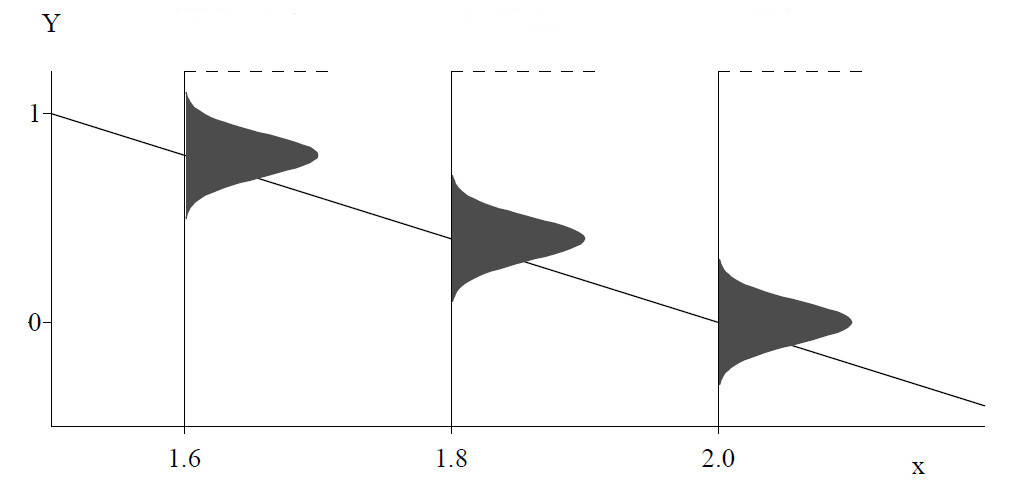
\includegraphics[width=0.7\textwidth,height=\textheight]{regrAssumptions.jpg}

\end{frame}

\begin{frame}

\begin{block}{Do-it-yourself ``by hand''}

\vspace{6mm}

Her kan du finne de beste parametrene selv: \vspace{2mm}

Bruk denne lenken: \vspace{2mm}

\url{https://gallery.shinyapps.io/simple_regression/}

\end{block}

\end{frame}

\begin{frame}{Multippel linear regresjon}
\protect\hypertarget{multippel-linear-regresjon}{}

Nesten det samme some enkel linear regresjon, vi bare summerer flere
forklaringsvariabler:

\[Y_i = \beta_0 + \beta_1 x_{1i} + \beta_2 x_{2i} + \ldots + \beta_p x_{pi} + e_i \ , \quad e_i \sim\mathsf{N}(0,\sigma^2) \ .\]
\(~\)

For eksempel:

\[\text{bodyfat}_i = \beta_0 + \beta_1 \text{bmi}_i + \beta_2 \text{age}_i + e_i \ .\]

\end{frame}

\begin{frame}

\centering

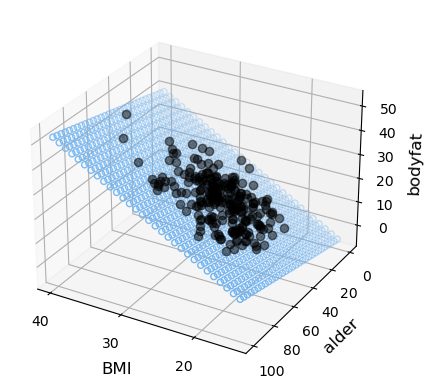
\includegraphics[width=0.7\textwidth,height=\textheight]{multippelRegGraph.png}

\end{frame}

\begin{frame}{Regresjonsanalyse i fem steg}
\protect\hypertarget{regresjonsanalyse-i-fem-steg}{}

\(~\)

\textbf{Steg 1}: Bli kjent med dataene ved å se på oppsummeringsmål og
ulike typer plott

\textbf{Steg 2}: Spesifiser en matematisk modell

\textbf{Steg 3}: Tilpass modellen

\textbf{Steg 4}: Presenter resultater fra den tilpassede modellen

\textbf{Steg 5}: Evaluer om modellen passer til dataene

\(~\)

Vi skal ikke snakke så mye om hvordan finne en god modell, men om
hvordan sammenligne to modeller (med justert \(R^2\)) .

\end{frame}

\begin{frame}

\begin{block}{Steg 1: Bli kjent med dataene}

\(~\)

Vi kan for eksempel se på histogram og boxplot:

\(~\)

\begin{center}\includegraphics[width=0.75\linewidth]{1Regresjon_files/figure-beamer/unnamed-chunk-1-1} \end{center}

\end{block}

\end{frame}

\begin{frame}

Ellers en \emph{parplot} med kryssplotter for alle
forklaringsvariable(r) \((x_1,\ldots, x_p)\) og respons \(y\):

\(~\)

\begin{center}\includegraphics[width=0.75\linewidth]{1Regresjon_files/figure-beamer/plots-1} \end{center}

\end{frame}

\begin{frame}[fragile]

\scriptsize

\begin{verbatim}
##     bodyfat           age            weight           height     
##  Min.   : 0.70   Min.   :22.00   Min.   : 56.75   Min.   :162.6  
##  1st Qu.:12.50   1st Qu.:35.50   1st Qu.: 72.30   1st Qu.:173.7  
##  Median :19.20   Median :43.00   Median : 80.02   Median :177.8  
##  Mean   :19.11   Mean   :44.83   Mean   : 80.91   Mean   :178.5  
##  3rd Qu.:25.20   3rd Qu.:54.00   3rd Qu.: 89.32   3rd Qu.:183.5  
##  Max.   :47.50   Max.   :81.00   Max.   :119.29   Max.   :196.8  
##       bmi             neck          abdomen            hip        
##  Min.   :19.06   Min.   :31.10   Min.   : 70.40   Min.   : 85.30  
##  1st Qu.:23.07   1st Qu.:36.40   1st Qu.: 84.90   1st Qu.: 95.55  
##  Median :25.10   Median :38.00   Median : 91.00   Median : 99.30  
##  Mean   :25.34   Mean   :37.96   Mean   : 92.38   Mean   : 99.69  
##  3rd Qu.:27.34   3rd Qu.:39.40   3rd Qu.: 99.15   3rd Qu.:103.15  
##  Max.   :39.12   Max.   :43.90   Max.   :126.20   Max.   :125.60
\end{verbatim}

\(~\)

\normalsize

I Python får du en oppsummering av datasettet (\texttt{df}) med
\texttt{df.describe()}.

\end{frame}

\begin{frame}[fragile]

\begin{block}{Steg 2: Spesifiser modell}

\(~\)

Nå må vi spesifisere en modell med å velge hvilke forklaringsvariabler
vi vil bruke

\[ y \sim x_1 + x_2 + x_3 \ .\]

\vspace{2mm}

I Python er det

\vspace{2mm}

\centering

\texttt{formel=\textquotesingle{}y\ \textasciitilde{}\ x1\ +\ x2\ +\ x3\textquotesingle{}}.

\end{block}

\end{frame}

\begin{frame}[fragile]

\textbf{Eksempel 1}:

\[\text{bodyfat} \sim \text{bmi} \] hvis den matematiske modellen er
\[\text{bodyfat}_i = \beta_0 + \beta_1 \text{BMI}_i + e_i \ , \] Python:
\texttt{formel=\textquotesingle{}bodyfat\ \textasciitilde{}\ bmi\textquotesingle{}}.

\(~\)

\textbf{Eksempel 2}:

\[\text{bodyfat} \sim \text{bmi} + \text{age}\] hvis den matematiske
modellen er
\[\text{bodyfat}_i = \beta_0 + \beta_1 \text{BMI}_i + \beta_2 \text{age}_i + e_i \ . \]

Python:
\texttt{formel=\textquotesingle{}bodyfat\ \textasciitilde{}\ bmi\ +\ age\textquotesingle{}}.

\end{frame}

\begin{frame}

\begin{block}{Steg 3: Tilpass modellen}

\(~\)

``Tilpasse'' betyr:

\(~\)

\begin{itemize}
\tightlist
\item
  Vi estimerer \(\beta_0\), \(\beta_1\), \ldots{} , og vi får estimater
  \(\hat\beta_0\), \(\hat\beta_1\),\ldots{}
\end{itemize}

\(~\)

\begin{itemize}
\tightlist
\item
  I tillegg estimerer vi også \(\sigma^2\).
\end{itemize}

\end{block}

\end{frame}

\begin{frame}

\begin{block}{Steg 4: Resultat og tolkning av estimatene}

\(~\)

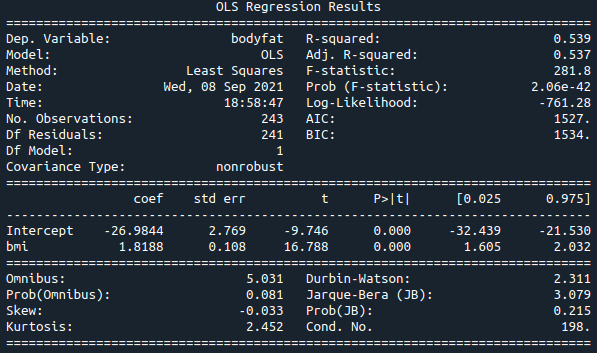
\includegraphics[width=0.7\textwidth,height=\textheight]{ols_result.png}

\vspace{20mm}

\end{block}

\end{frame}

\begin{frame}

\begin{itemize}
\item
  Tilpasset regressjonslinie og 95\% konfidensintervall for
  regressjonslinia (forventningsverdien \(\text{E}(Y)\)).
\item
  95\% prediksjonsintervall for nye observasjoner (kroppsfett for nye
  personer; handtegnet)
\end{itemize}

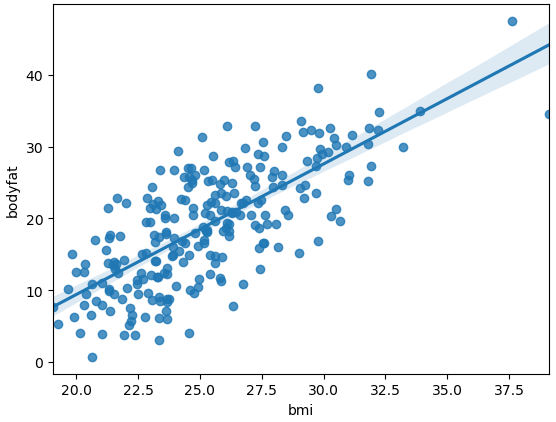
\includegraphics[width=0.7\textwidth,height=\textheight]{ols_result_plot.png}

\end{frame}

\begin{frame}

\begin{block}{Steg 5: Passer modellen?}

\(~\)

\textbf{Tukey-Anscome (TA) diagram}:

\(~\)

\centering

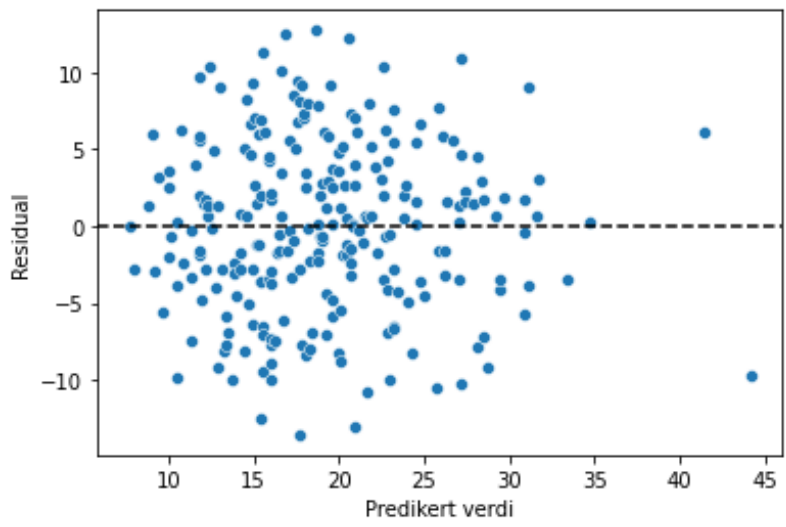
\includegraphics[width=0.6\textwidth,height=\textheight]{tukeyAnscombe1.png}

\flushleft

Her vil man

\begin{itemize}
\tightlist
\item
  Ikke noe struktur
\item
  Sentrering rundt 0 verdi
\end{itemize}

\end{block}

\end{frame}

\begin{frame}

\(~\)

\textbf{Kvantil-kvantil plot}:

\(~\)

\centering

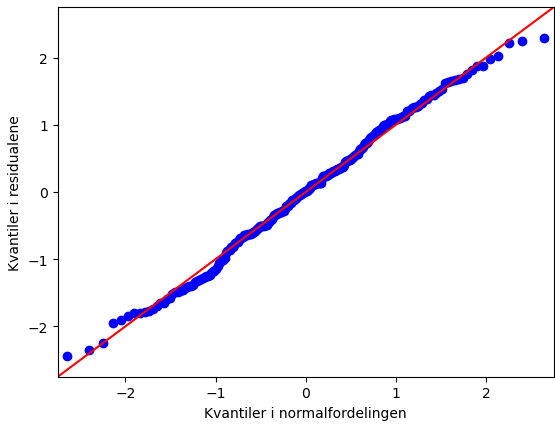
\includegraphics[width=0.6\textwidth,height=\textheight]{kvantilplot.png}

\flushleft

Her vil man at observasjoner ligger mer og mindre på linja.

\end{frame}

\begin{frame}

Hvordan ser det ut når en modell \emph{ikke} passer?

\begin{center}\includegraphics[width=0.75\linewidth]{1Regresjon_files/figure-beamer/unnamed-chunk-4-1} \end{center}

\end{frame}

\begin{frame}[fragile]

\begin{block}{Multippel linear regresjon}

\(~\)

Gjenta samme analyse med to kovariabler\\
(\texttt{formel=\textquotesingle{}bodyfat\ \textasciitilde{}\ bmi\ +\ age\textquotesingle{}}):

\(~\)

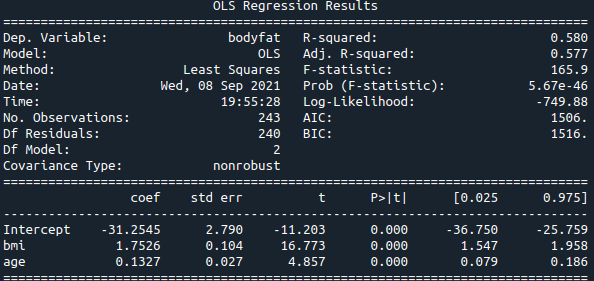
\includegraphics[width=0.7\textwidth,height=\textheight]{ols_result_2.png}

\vspace{20mm}

\end{block}

\end{frame}

\begin{frame}[fragile]

Med fem kovariabler:

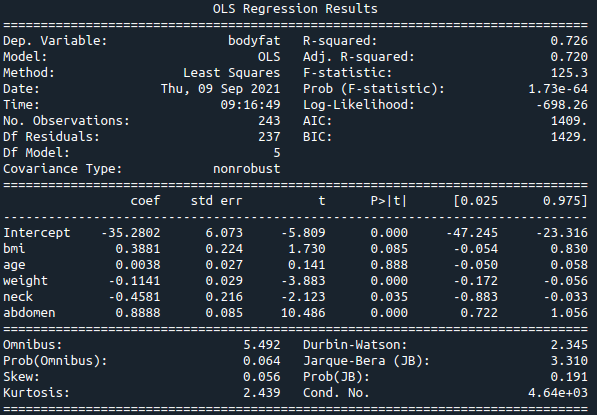
\includegraphics[width=0.65\textwidth,height=\textheight]{ols_result_all.png}

Hva betyr alt dette?

\begin{itemize}
\tightlist
\item
  \texttt{coef}: \(\hat\beta_j\)
\item
  \texttt{std\ err}: \(\hat\text{SE}(\hat\beta_j)\)
\item
  \texttt{t}: \(\frac{\hat\beta_j-0}{\text{SE}(\hat\beta_j)}\)
\item
  \texttt{P\textgreater{}\textbar{}t\textbar{}}: \(p\)-verdi (obs!
  \(p=0.000\) er \emph{ikke} mulig, det betyr egentlig \(p<0.001\))
\end{itemize}

\end{frame}

\begin{frame}[fragile]

\begin{block}{Hva betyr alt dette?}

\vspace{2mm}

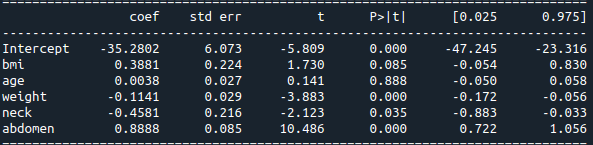
\includegraphics[width=0.7\textwidth,height=\textheight]{ols_result_all_coefs.png}

\vspace{2mm}

Prediksjon:

\vspace{2mm}

\(\hat{y}=\)

\vspace{10mm}

Prediker bodyfat for en ny person med\\
\texttt{bmi=25}, \texttt{age=50}, \texttt{weight=75}, \texttt{neck=40},
\texttt{abdomen=95}:

\vspace{2mm}

\(\hat{y}=\)

\(~\)

= 21.88

\end{block}

\end{frame}

\begin{frame}

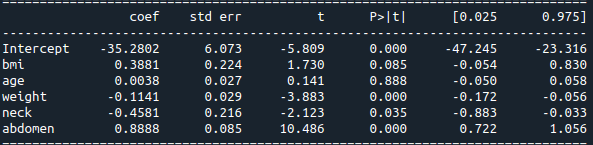
\includegraphics[width=0.7\textwidth,height=\textheight]{ols_result_all_coefs.png}

\vspace{2mm}

\begin{itemize}
\item
  Hva betyr \(\hat\beta_0\)?
\item
  Hva betyr \(\hat\beta_{abdomen}=0.89\)?
\end{itemize}

\vspace{20mm}

\end{frame}

\begin{frame}

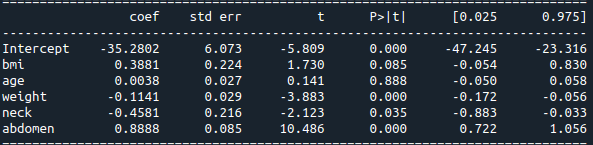
\includegraphics[width=0.7\textwidth,height=\textheight]{ols_result_all_coefs.png}

\vspace{5mm}

\begin{itemize}
\item
  95\% konfidensintervall: Intervall vi har stor tro at den inneholder
  den sanne \(\beta_j\).
\item
  \([\hat\beta_j \pm \underbrace{t_{\alpha/2,df}}_{\approx 1.96}\cdot \text{SE}(\hat\beta_j)]\)
\end{itemize}

\vspace{20mm}

\end{frame}

\begin{frame}

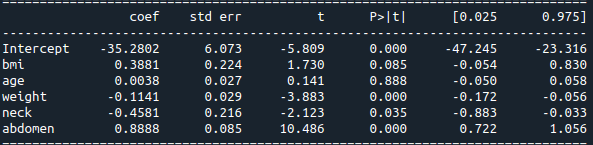
\includegraphics[width=0.7\textwidth,height=\textheight]{ols_result_all_coefs.png}

\vspace{5mm}

\begin{itemize}
\tightlist
\item
  \(p\)-verdier og hypotesetester
\end{itemize}

\vspace{20mm}

\end{frame}

\begin{frame}

\begin{block}{Recap: Formell definisjon av \(p\)-verdien}

\(~\)

\textbf{\(p\)-verdien} er sannsynligheten for det vi \emph{har}
observert eller noe mer ekstremt, dersom \(H_0\) er sant.

\vspace{5mm}

\begin{center}\includegraphics[width=1\linewidth]{1Regresjon_files/figure-beamer/pValFig2-1} \end{center}

\end{block}

\end{frame}

\begin{frame}

\begin{block}{\(R^2\) og justert \(R^2\)}

\(~\)

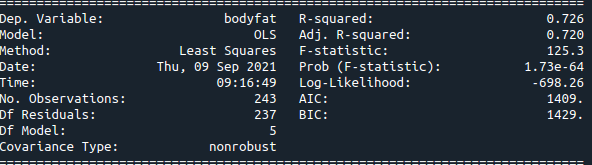
\includegraphics[width=0.7\textwidth,height=\textheight]{ols_result_all_header.png}

\[R^2 = \frac{\text{TSS}-\text{SSE}}{\text{TSS}}= 1-\frac{\text{SSE}}{\text{TSS}}=1-\frac{\sum_{i=1}^n(y_i-\hat{y}_i)^2}{\sum_{i=1}^n(y_i-\bar{y}_i)^2}, \]

med \[\text{TSS} = \sum_{i=1}^n (y_i - \bar{y})^2\] som måler den totale
variabiliteten i \((y_1,\ldots , y_n)\).

\vspace{2mm}

\end{block}

\end{frame}

\begin{frame}

Problemet med \(R^2\): Verdien blir alltid større når flere variabler er
lagt til.

\(~\)

For modellvalg bruker vi derfor en justert versjon:

\[R^2_{adj} = 1-(1-R^2 )\frac{n-1}{n-m-1}\]

\end{frame}

\begin{frame}

\begin{block}{TA og kvantil-kvantil plot}

\(~\)

\(~\)

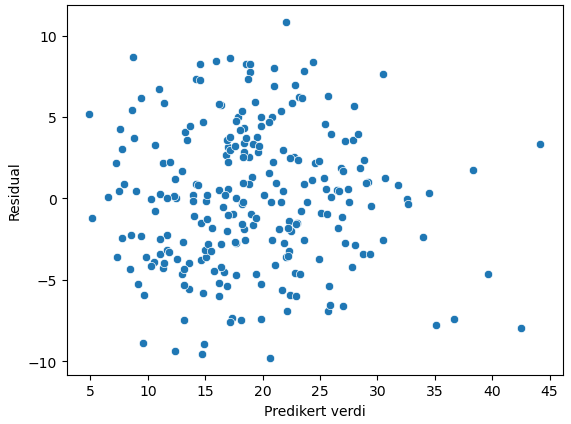
\includegraphics[width=0.47\textwidth,height=\textheight]{ta2.png}
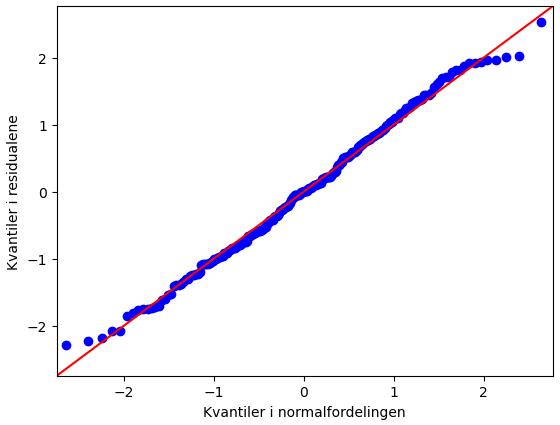
\includegraphics[width=0.42\textwidth,height=\textheight]{qq2.png}

\end{block}

\end{frame}

\begin{frame}

\begin{block}{Binære forklaringsvariabler}

\(~\)

Den enkleste modellen er

\[y_i = \beta_0 + \beta_1 x_{1i} + e_i \ .\] \(~\)

Hva betyr det når \(x_{1i}\) er enten 0 eller 1 (binær)?

\[
\begin{array}{ll}
 \beta_0  + e_i \quad &\text{ hvis  } x_{1i}=0 \\
 \beta_0 + \beta_1 + e_i \quad &\text{ hvis  } x_{1i} =1\\
\end{array}
\]

\end{block}

\end{frame}

\begin{frame}

\begin{block}{Eksempel: Studie om kvikksølv (Hg)}

\(~\)

Modell:

\[
\log(Hg_{urin})_i  = \beta_0 +  \beta_1 \cdot x_{1i} +  \beta_2\cdot x_{2i} + \beta_3 \cdot x_{3i} + e_i \ ,
\] \(~\)

Med

\begin{itemize}
\tightlist
\item
  \(\log(Hg_{urin})\): log konsentrasjon av Hg i urin.
\item
  \(x_{1}\) binær variabel som er 1 hvis person røyker, ellers 0.
\item
  \(x_{2}\) antall amalgam fillinger i tennene
\item
  \(x_{3}\) antall fiskemåltider per måned.
\end{itemize}

\end{block}

\end{frame}

\begin{frame}

\begin{block}{Interpretasjon av regresjon med binær variabel}

\(~\)

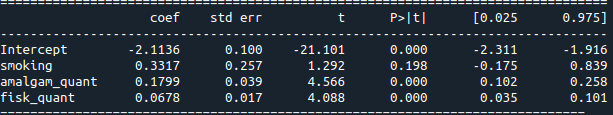
\includegraphics[width=0.8\textwidth,height=\textheight]{binaer_variabel.png}

\(~\)

Modell for røyker:

\vspace{15mm}

Modell for ikke-røyker:

\end{block}

\end{frame}

\begin{frame}[fragile]

\begin{block}{Kategoriske forklaringsvariabler}

\(~\)

\begin{itemize}
\tightlist
\item
  Vi gjør ting enda mer fleksibel (eller komplisert!) når vi også
  tillater kategoriske forklaringsvariabler.
\end{itemize}

\vspace{2mm}

\begin{itemize}
\tightlist
\item
  Eksempel med 3 kategorier: Bil dataset med \(y\)=bensinforbruk og
  forklaringsvariabler \texttt{vekt} og
  \texttt{origin}\(\in \{\text{American,European,Japanese}\}\).
\end{itemize}

\centering

\vspace{4mm}

\texttt{formel=\textquotesingle{}mpg\ \textasciitilde{}\ \ vekt\ +\ origin\textquotesingle{}}

\flushleft

\vspace{4mm}

\begin{itemize}
\item
  Ide: dummy-variabel koding -- kalles \emph{one-hot koding} i
  maskinlæring.

  \begin{itemize}
  \tightlist
  \item
    \(x_{2i}=0\) og \(x_{3i}=0\) hvis \texttt{origin} er ``American''
  \item
    \(x_{2i}=1\) og \(x_{3i}=0\) hvis \texttt{origin} er ``European''
  \item
    \(x_{2i}=0\) og \(x_{3i}=1\) hvis \texttt{origin} er ``Japanese''
  \end{itemize}
\end{itemize}

\vspace{4mm}

Modellen:
\(y_i = \beta_0 + \beta_1 x_{1i} + \beta_2 x_{2i} + \beta_3 x_{3i} + e_i\)

\end{block}

\end{frame}

\begin{frame}[fragile]

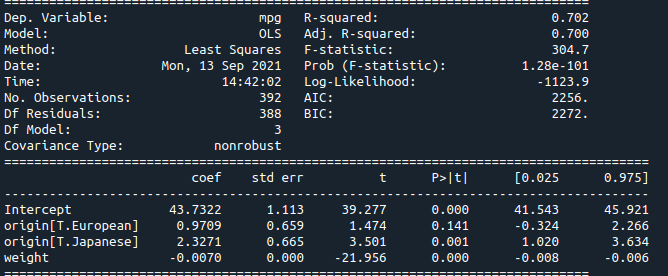
\includegraphics{kategorisk_variabel.png}

\vspace{2mm}

Så hva er modellene for de tre opprinnelsene (\texttt{origin}) av
bilene?

\end{frame}

\begin{frame}{Videre denne uken}
\protect\hypertarget{videre-denne-uken}{}

\(~\)

\begin{itemize}
\tightlist
\item
  Se på videoene om multippel linear regresjon (hvis du ikke har
  allerede gjort det).
\end{itemize}

\(~\)

\begin{itemize}
\tightlist
\item
  Se på videoene om klassifikasjon.
\end{itemize}

\(~\)

\begin{itemize}
\tightlist
\item
  Les i kompendiet
\end{itemize}

\(~\)

\begin{itemize}
\tightlist
\item
  Begynn å jobbe med prosjektoppgavene -- problem 1
\end{itemize}

\(~\)

\begin{itemize}
\tightlist
\item
  Se her for mer informasjon:
  \url{https://wiki.math.ntnu.no/istx1003/2021h/start}
\end{itemize}

\end{frame}

\end{document}
